\documentclass{beamer}

\usetheme[secheader]{Boadilla}
\usecolortheme{beaver}
\usepackage[spanish]{babel}
\usepackage{ragged2e}
\usepackage{xfrac}

%Definicion del color de los bloques que contienen texto
\setbeamercolor{block title}{bg=gray!60,fg=black}

%IGNORAR - Template de la portada
\defbeamertemplate*{title page}{Cony}
{
	\vspace{-8ex}
	\hspace{-3ex}
	% Header UC, versi�n IEE
	\hbox
	{
		\raisebox{-18pt}{
\includegraphics[scale=0.65]{logo.pdf}}
		\vbox
		{
			\hbox{\small \insertinstitute} 
			\hbox{\small \college}
			\hbox{\small \department}
		}	
	}
  \vspace{5ex}
  \begin{block}{}
  \center{
    \usebeamercolor[fg]{title}\usebeamerfont{title}\inserttitle\par
    \usebeamercolor[fg]{subtitle}\usebeamerfont{subtitle}\insertsubtitle
    }
  \end{block}
  \ifx\insertauthor\@empty
  \else
    \center{\usebeamercolor[fg]{author}\usebeamerfont{author}\insertauthor\par}
  \fi
  \ifx\insertdate\@empty
  \else
   \center{\usebeamercolor[fg]{date}\usebeamerfont{date}\insertdate\par}
  \fi
}
%DEJAR DE IGNORAR

\title{IEE3724 Reconocimiento de Patrones}
\subtitle{Proyecto - Entrega 1}
%El string entre brackets se incluye en el pie de p�gina, el resto en la portada.
\author[C. Villanueva - R. Gonz\'alez]{Constanza Villanueva - Rodrigo Gonz\'alez}
\date{Mayo 15, 2014}
%Rellenar el espacio entre brackets para incluir informaci�n junto al nombre
%del autor en los pies de p�gina.
\institute[]{Pontificia Universidad Cat\'olica de Chile}
\def\college{Escuela de Ingenier\'ia}
\def\department{Departamento de Ingenier\'ia El\'ectrica}

%La siguiente l�nea elimina los s�mbolos de navegaci�n que aparecen
%en la zona inferior derecha del documento. Queda mejor para una
%presentaci�n pero puede ser �til para una clase.
\setbeamertemplate{navigation symbols}{}

%Color y estilo de vi�etas
\setbeamertemplate{itemize item}{\color{red!70!black}$\bullet$}
\setbeamertemplate{itemize subitem}{\color{red!70!black}$\blacktriangleright$} 
%Tambi�n se puede usar \circ u otros s�mbolos
\setbeamercolor{enumerate item}{fg=red!70!black}
\setbeamercolor{enumerate subitem}{fg=red!70!black}
\setbeamertemplate{enumerate items}[default]
\setbeamertemplate{enumerate subitems}[default]

%INICIO DEL PPT
\begin{document}

%Portada
\frame{\titlepage}

%Tabla de contenidos
%\section[Contenidos]{}
%\frame{\tableofcontents}

\section{Reconocimiento de G\'eneros Musicales}
\subsection{Definici\'on del Proyecto}
\frame {
	\frametitle{Reconocimiento de G\'eneros Musicales}
	\begin{itemize}
	\justifying
	\item Objetivos\\
	La m\'usica es un elemento que se encuentra en gran cantidad en la web hoy en d\'ia. La clasificaci\'on de esta seg\'un su g\'enero es un herramienta muy utilizada para algoritmos de b\'usqueda y categorizaci\'on.
	\begin{itemize}
	\justifying
	\item Se desea desarrollar, en vista de lo anterior, un programa que permita identificar el g\'enero musical de una pista de audio, de un conjunto preseleccionado de clases.
	\item Se debe elegir un conjunto apropiado de \textit{Feature Vectors} que permita analizar los distintos componentes que definen un g\'enero de otro.
	\item La elecci\'on del g\'enero particular de cada audio es muy suceptible a ambig\"{u}edades, ya que una canci\'on puede tener mezcla de g\'eneros y el g\'enero principal elegido en los labels utilizados puede ser por elecci\'on personal. En vista de esto hay que tener en cuenta posible subclasificaciones como m\'etodo de exteneder la clasificaci\'on.
	\end{itemize}
	\end{itemize}
	
}

\frame {
	\frametitle{Esquema del Programa a Implementar}
	\begin{itemize}
	\justifying
	\item Para implementar el programa se utilizar\'a Matlab.
	\item La entrada al programa ser\'an las pistas de audio en conjunto con los \textit{labels} de las clases, tanto para los sets de entrenamiento como para los de validaci\'on y testeo.
	\item Se analizar\'a el uso de distintos tipos de \textit{Features} en distintas combinaciones, adem\'as de comparar m\'etodos de clasificaci\'on.
	\item La salida del programa entregar\'a las matrices de confusi\'on de las distintas pruebas.
	\end{itemize}
	
	
}

\frame {
	\frametitle{Restricciones}
	\begin{itemize}
	\justifying
	\item\textbf{ Formato de Audio:}	Se trabajar\'a con audio en los siguientes posibles formatos: MP3, WAV y AU. En general, se buscan formatos que permitan una buena calidad de audio y que no sea necesaria una conversi\'on extra para su trabajo en Matlab. En ese sentido no se trabajar\'a con audios monof\'onicos como los en formato MIDI.
	\item\textbf{ Duraci\'on de las pistas:}	El largo de las pistas puede ser cualquiera, pudiendo utilizarse tanto el total de la canci\'on, lo que permitir\'a un mayor an\'alisis de ventanas, como trozos de las pistas. La restricci\'on ira en que la m\'inima duraci\'on a trabajar es de 10 segundos.
%	\item Calidad del audio: Debido a temas de \textit{Copyright}, es complicado conseguir audio de forma l'egitima. Para esto se puede utilizar grabaciones de audio que podr\'ian as\'i representar un mayor reto respecto al an\'alisis de estas pistas frente al ruido de la grabaci\'on.
	\item\textbf{ Clases:} El programa solo ser\'a capaz de analizar g\'eneros musicales de un conjunto determinado de clases, cualquier otro g\'enero ser\'a clasificado seg\'un su aproximaci\'on m\'as cercana a los g\'eneros disponibles.
	\end{itemize}
	
}

\frame {
	\frametitle{Metodolog\'ias Actuales}
	\justifying
	Existen en la literatura actual diversos tipos de caracter\'isticas para el an\'alisis de se\~nales de audio, entre estos grupos destacan:
	\begin{itemize}
	\justifying
	\item \textbf{Caracter\'isticas Temporales:}\\
	Se basan en el estudio de la se\~nal en el dominio del tiempo como son los c\'alculos de energ\'ia y raz\'on de cruces por cero.
	\item \textbf{Caracter\'isticas Espectrales:}\\
	Corresponde al grupo m\'as desarrollado de caracter\'isticas donde se analiza el contenido en frecuencia de la se\~nal. Por un lado, existen caracter\'isticas simples, como el c\'alculo del centroide espectral, la uniformidad del espectro, su tasa de crestas o bien el flujo espectral.\\
	Por otro lado, existen otras m\'as complejos, como veremos adelante, correspondientes a los cepstrum, los que permiten an\'alisis del contenido harm\'onico.
	\item \textbf{Caracter\'isticas R\'itmicas:}\\
	Una mezcla de ambos aspectos anteriores con el fin de determinar detalles r\'itimicos, como son el tempo o \textit{beat histograms}.
	\end{itemize}
}

\subsection{Estado del Arte}
\frame {
	\frametitle{Metodolog\'ias Actuales}
	\justifying
	\begin{itemize}
	\item \textbf{\textit{``Music Genre Classification Algorithm Based on Dynamic Frame Analysis and Support Vector Machine"}}, Shih-Hao \textit{et al.}\vspace{1ex}\\
	En base a estudios psicof\'isicos previos, se conoce que la percepci\'on humana del contenido en frecuencia de una se\~nal sigue una funci\'on no lineal, llamada la escala de \textit{mel}, donde:
	\begin{equation*}
	f_{mel} = 1125 \ln\left(1 + \dfrac{f}{700}\right)
	\end{equation*}
	\vspace{-3.5ex}
	\begin{center}
  	\begin{minipage}{5cm}
  	  	\begin{center}
  	  		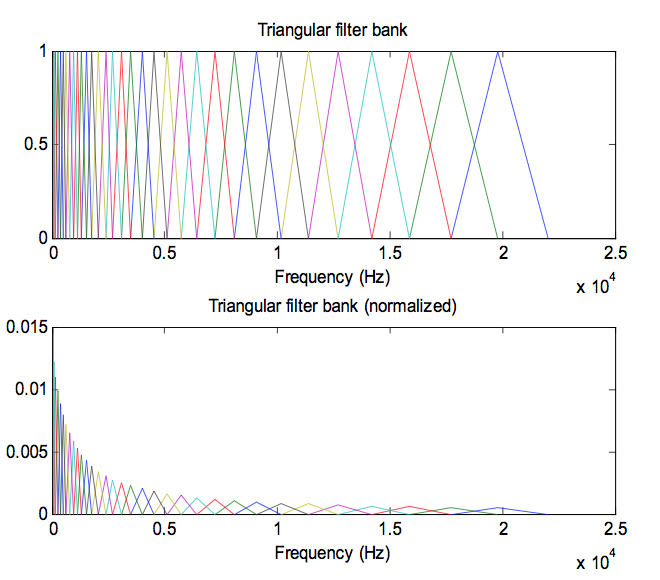
\includegraphics[scale=0.42]{TriangularFilterBank.png}
  	  	\end{center}
  	\end{minipage}
  	\begin{minipage}{6cm}
  	Con lo anterior, es posible dise\~nar un banco filtros pasabanda linealmente espaciados en la representaci\'on de \textit{mel} que, al filtrar una se\~nal, se espera segmenten contenido de igual percepci\'on en frecuencia.
  	\end{minipage}
  	\end{center}
	\end{itemize}
}

\frame {
	\frametitle{Metodolog\'ias Actuales}
	\justifying
	El principal conjunto de caracter\'isticas a obtener de la respuesta de la se\~nal a cada filtro de frecuencias de \textit{mel}, $e_i[m]$, son los coeficientes cepstrales:
	\begin{equation*}
	C_i = \sqrt{\dfrac{2}{N}}\sum \limits_{n = 0}^{N-1} \ln{e_i[n+1]}\cos{\left[i \left(\dfrac{2n-1}{2}\right) \dfrac{\pi}{N}\right]}
	\end{equation*}
	En forma general, el cepstrum corresponde a la transformada de Fourier discreta del logaritmo natural de una funci\'on en frecuencia. En este paper utilizan DCT en vez de FT. \vspace{1ex}\\ 
	En la se\~nal resultante, los coeficientes $C_i$ de mayor magnitud representar\'an la existencia de harm\'onicos peri\'odicos de magnitud $\sfrac{f_s}{C_i}$ en el espectro original, donde $f_s$ es la frecuencia de muestro de la se\~nal (e.g. $44100Hz$ en audio). \vspace{1ex}\\
	Este vector de features se conoce como \textbf{Mel-Frequency Cepstral Coefficients (MFCC)}.
}

\frame {
	\frametitle{Metodolog\'ias Actuales}
	\justifying
	En el paper de Shih-Hao \textit{et al.} se ocupan las caracter\'isticas anteriores calculadas en \textbf{ventana din\'amicas de Hamming}, las que permiten analizar la se\~nal por tramos enfatizando las magnitudes del centro de la se\~nal recortada.�\vspace{1ex}\\
	Respecto de la clasificaci\'on, el conjunto de \textit{features} extra\'idos es procesado por un clasificador SVM no lineal, pues se corrobor\'o que un \textbf{Kernel exponencial de base radial (ERBF)} maximizaba la precisi\'on del algoritmo.\vspace{1ex} \\
	Dado que el clasificador SVM esta dise\~nado para clasificar entre dos clases, se opt\'o por un clasificador compuesto para an\'alisis \textbf{uno-contra-uno} para cada par de clases, en vez de un formato uno-contra-todos.\vspace{1ex} \\
	El conjunto de clases dadas por los distintos g\'eneros musicales contenidos en el dataset utilizado fueron $\{classical, dance, lullaby, bossa, piano, blues\}$. Con todo lo anterior se logr\'o una precisi\'on del $98\%$ al entrenar con $45$ canciones de un total de $300$.
}


\frame {
	\frametitle{Metodolog\'ias Actuales}
	\begin{itemize}
	\justifying
	\item \textbf{\textit{``Music Genre Classification Using GA-Induced Minimal Feature-Set"}}, Nayak \& Bhutani.\vspace{1ex}\\
	Es posible hallar un set m\'inimo y \'optimo de caracter\'isticas a utilizar en la clasificaci\'on de g\'eneros musicales.\vspace{1ex}\\ Para ello se utiliza un algoritmo gen\'etico, con recombinaci\'on y mutaci\'on aleatorias, que modela en cada bit de los cromosomas la utilizaci\'on o no de una caracter\'istica espec\'ifica.
	\begin{center}
	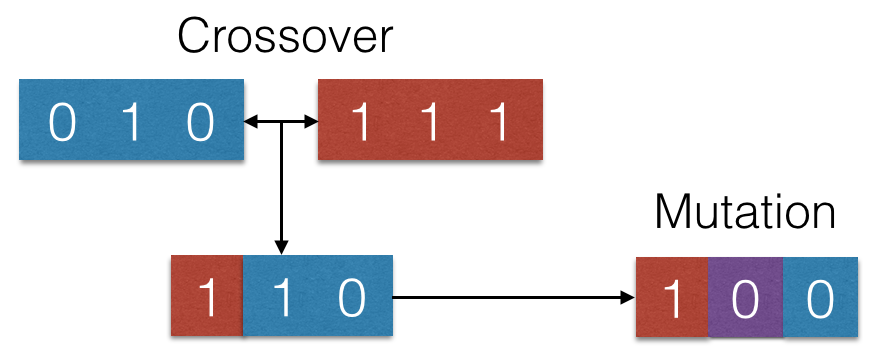
\includegraphics[scale=0.4]{GeneticProcess.png}
	\end{center}
	\end{itemize}
}

\frame {
	\frametitle{Metodolog\'ias Actuales}
	\justifying
	La selecci\'on de cromosomas en cada etapa se realizar por una funci\'on de \textit{fitness} del tipo:
	\begin{equation*}
	Fitness = HR + \gamma(\sfrac{CD}{p}) + \beta(\sfrac{c}{p})
	\end{equation*}
	donde se tiene:
	\begin{itemize}
	\item $HR$: \textit{Hit-rate}, es decir, la fracci\'on de datos de entrenamiento correctamente clasificados.
	\item $CD$: distancia entre clases, para evitar m\'inimos locales por $HR$.
	\item $p$: n\'umero de muestras.
	\item $c$: n\'umero de ceros en el cromosoma, es decir, caracter\'isticas no usadas.
	\item $\gamma, \beta$: factores de escalamiento, importancia de la separaci\'on de clases y de la minimizaci\'on de caracter\'isticas, respectivamente.
	\end{itemize}
}

\frame {
	\frametitle{Metodolog\'ias Actuales}
	\begin{itemize}
	\justifying
	\item \textbf{\textit{``Feature Mapping and Fusion for Music Genre Classification"}}, Balti \& Frigui.
\begin{center}
  	\begin{minipage}{3.5cm}
	Se presenta un concepto similar al \textit{bag of words} donde las caracter\'isticas se asocian en subconjuntos y, para cada uno, se obtiene una clusterizaci\'on de las $K$ clases.
  	\end{minipage}
  	\begin{minipage}{7.5cm}
  	  	\begin{center}
  	  		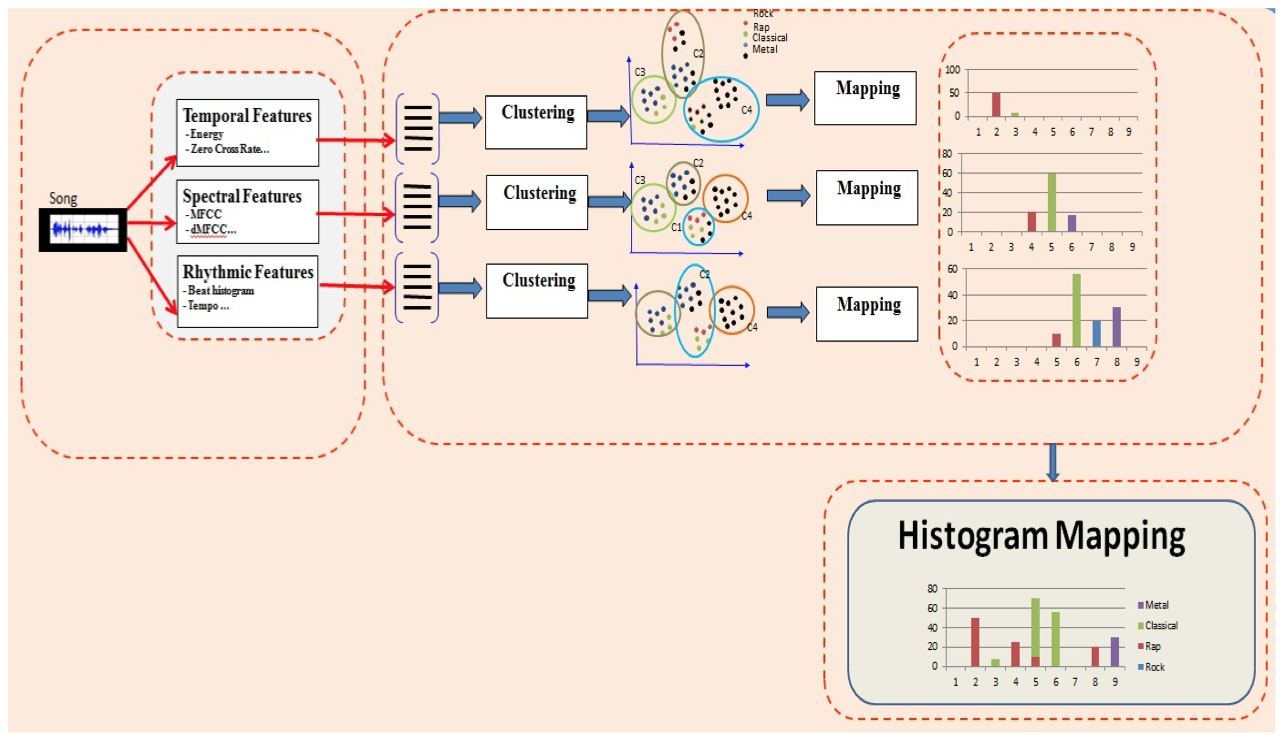
\includegraphics[scale=0.30]{HistogramMapping.png}
  	  	\end{center}
  	\end{minipage}
  	\end{center}
	Luego, para cada cluster se genera una funci\'on de pertenencia gaussiana en torno al centro, la cual permite realizar un \textit{soft assignment} con el cual generar un histograma normalizado, en base a datos de entrenamientos, que se utiliza como vector de caracter\'isticas final.
	\end{itemize}
}

\frame {
	\frametitle{Metodolog\'ias Actuales}
	\begin{itemize}
	\justifying
	\item \textbf{\textit{``Music genre recognition based on visual features with dynamic ensemble of classifiers selection"}}, Costa \textit{et al}.\\
	Las pistas de audio son convertidas a su correspondiente espectro en frecuencia, la imagen obtenida se utiliza como base de an\'alisis. Se utilizan ventanas de audio en lugar de analizar el audio completo.\\
	El entrenamiento se hace utilizando SVM entrenada con texturas utilizando LBP. El avance principal de este estudio se base en generar un conjunto din\'amico de clasificadores que se ajusta a cada zona extraida del espectro.
	\begin{center}
	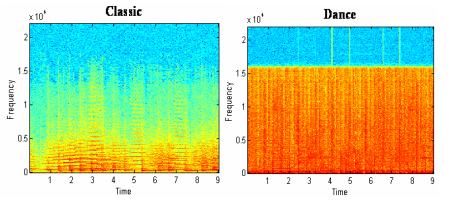
\includegraphics[scale=0.6]{espectro.png}
	\end{center}

	\end{itemize}
}

\subsection{Enfoque de Trabajo}
\frame {
	\frametitle{Metodolog\'ia a Investigar}
	La metodolog\'ia que hemos decidido utilizar se compone por varias etapas presentadas en el siguiente diagrama.
	\begin{center}
	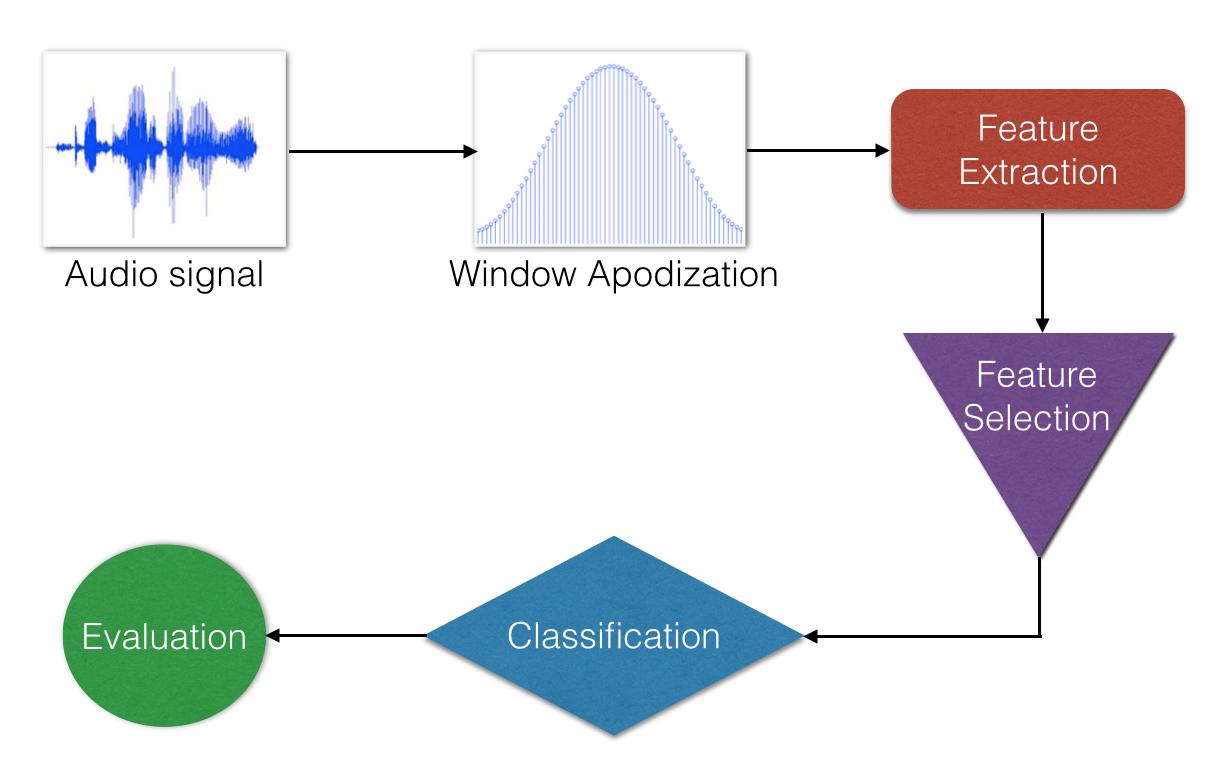
\includegraphics[scale=0.4]{EsquemaV2.png}
	\end{center}
	
}

\subsection{Enfoque de Trabajo}
\frame {
	\frametitle{Metodolog\'ia a Investigar}
	Para cada una de las etapas se considera utilizar los siguientes algoritmos:
	\begin{enumerate}
	\justifying
	\item \textbf{Window Apodization:} ventana m\'ovil de 10 segundos con estructura de Hamming para el \'enfasis en valores centrales.
	\item \textbf{Feature Extraction:} Mel-Frequency Cepstral Coefficientes, energ\'ia de la se\~nal, frecuencia fundamental, Loudness Sensation, Integral Loudness, Zero Crossing Rate, entre otros.
	\item \textbf{Feature Selection:} Principal Componente Analysis; preferimos una soluci\'on determin\'istica antes de un algoritmo gen\'etico que pudiera inducir \'optimos locales y sesgar los resultados.
	\item \textbf{Classification:} Support Vector Machines, donde se probar\'a la diferenciaci\'on de clases en formato uno-contra-uno y uno-contra-todos. 
	\item \textbf{Evaluation:} Se considerar\'a tanto la precisi\'on en la clasificaci\'on por ventanas como en una pista de audio completa. El primer caso es el t\'ipico de la literatura mientras que el segundo es el necesario de implementar en softwares de m\'usica como son iTunes y Spotify.
	\end{enumerate}
	
}

\subsection{Datasets}
\frame {
	\frametitle{Datasets a Utilizar}
	\begin{itemize}
	\justifying
	\item \textbf{GTZAN Genre Collection}\\
	Este Dataset es utilizado en varios de los papers investigados. Consta de 1000 pistas de audio de 30 segundos cada una. La clasificaci\'on esta hecha sobre 10 g\'eneros, por lo que hay 100 pistas por g\'enero. El formato de estas pistas es .au	Los g\'eneros utilizados son:\\
	Rock, Reggae, Pop, Metal, Jazz, Hip-Hop, Disco, Country, Classical y  Blues. 
	%http://marsyas.info/download/data_sets/
	
	\item \textbf{Music Audio Benchmark Dataset}\\
	Este dataset consta de 1886 canciones en formato .mp3, donde nuevamente corresponden a una fracci\'on de la pista de 10 segundos. La cantidad de pistas por g\'enero no estan definidas. Las clases utilizadas son las siguientes:\\
	Alternative, Blues, Electronic, Folk-Country, Folk-Soul, Jazz, Pop, Rap Hip-Hop y Rock.
	%http://www-ai.cs.uni-dortmund.de/audio.html

	\end{itemize}
	
}

\subsection{Bibliograf\'ia}
\frame {
	\frametitle{Bibliograf\'ia}
	\begin{itemize}
	\small
	\item Shih-Hao Chen; Shi-Huang Chen; Guido, R.C.,\textit{``Music Genre Classification Algorithm Based on Dynamic Frame Analysis and Support Vector Machine''}, Multimedia (ISM), 2010 IEEE International Symposium on , vol., no., pp.357,361, 13-15 Dec. 2010
	\item Nayak, S.; Bhutani, A.,\textit{``Music Genre Classification Using GA-Induced Minimal Feature-Set''}, Computer Vision, Pattern Recognition, Image Processing and Graphics (NCVPRIPG), 2011 Third National Conference on , vol., no., pp.33,36, 15-17 Dec. 2011
	\item Balti, H.; Frigui, H., \textit{``Feature Mapping and Fusion for Music Genre Classification''}, Machine Learning and Applications (ICMLA), 2012 11th International Conference on , vol.1, no., pp.306,310, 12-15 Dec. 2012
	\item Costa, Y.; Oliveira, L.; Koerich, A.; Gouyon, F., \textit{``Music genre recognition based on visual features with dynamic ensemble of classifiers selection''}, Systems, Signals and Image Processing (IWSSIP), 2013 20th International Conference on , vol., no., pp.55,58, 7-9 July 2013
	\end{itemize}
	
}







\end{document}